%-----------------------------------To Be Updated for Classroom Examples--------------
\documentclass{ResumeDesignFormat1}
\usepackage[english]{babel}
\usepackage{marginnote}
\usepackage{tikz}
\usepackage{hyperref}
\usetikzlibrary{positioning}
\usetikzlibrary{backgrounds}
\usepackage{tkz-berge}
\usepackage{sectsty}
\sectionfont{\footnotesize}
\subsectionfont{\Large}
\subsubsectionfont{\large}
\paragraphfont{\lfootnotesize}
\usepackage{pagecolor}
\definecolor{c1}{rgb}{0.858, 0.188, 0.478}
\definecolor{c2}{RGB}{219, 48, 122}
\definecolor{c3}{cmyk}{0, 0.7808, 0.4429, 0.1412}
\definecolor{c4}{gray}{0.1}
\definecolor{c5}{RGB}{142, 68, 173}
\definecolor{blueish}{rgb}{0.565,0.886,1} 
\definecolor{greenish}{rgb}{0.565,1,0.886}
\definecolor{darkgray}{rgb}{0.15,0.15,0.15} 
\definecolor{lightgray}{rgb}{0.6,0.6,0.6}
\graphicspath{{Figures/}}

\begin{document}
\pagecolor{purple!2}
%-------------------------------------------------------------------------------------------%
%----------------------------------------Contact Information--------------------------------%
%-------------------------------------------------------------------------------------------%
%-------------------------------------------------------------------------------------------%
Jeff Cromwell PhD
Linked In: https://www.linkedin.com/in/jeff-cromwellphd/

\section{Introduction}
%----------------------------------------Figure1--------------------------------------------% 
%-------------------------------------------------------------------------------------------%
\centering
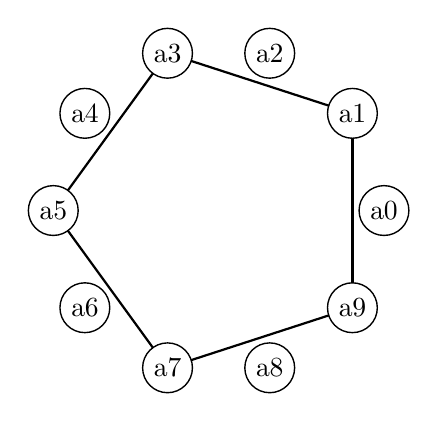
\begin{tikzpicture}[scale=0.35]
\grEmptyCycle[RA=6]{10}
\EdgeInGraphModLoop{a}{10}{2}{1}
\end{tikzpicture}
%-------------------------------------------------------------------------------------------%
%--------------------------------Summary----------------------------------------------------%
%-------------------------------------------------------------------------------------------%
\section{\centerline{\textcolor{c2}{Professional Summary}}}
%-------------------------------------------------------------------------------------------%
\input{/Summary/ProfessionalSummaryAcademic}
%-------------------------------------------------------------------------------------------%
%-------------------------------------------------------------------------------------------%
%----------------------------------------Jobs Section---------------------------------------%
%-------------------------------------------------------------------------------------------%
\section{Experience}
%---------------------------------------------------------------------------------------------------------------------------------%
%----------------------------Mathematical Learning Space--------------------------------------------------------------------------%
%---------------------------------------------------------------------------------------------------------------------------------%
\begin{enumerate}
\item {Weebly} {\href{http://mathlearningspace.weebly.com/}{\textcolor{c5}{Math Learning Space-Weebly}}}
\item {GitHib} {\href{https://github.com/MathematicalLearningSpace$}{ \textcolor{c5}{Mathematical Learning Space-GitHub}}}
\item {Math Numerical Projects}{ \textcolor{c2}{Development of the GitHub Mathematical Learning Space to Assist Students in Learning Applied Mathematics}}
\item {TMLS} {\href{http://mathlearningspace.weebly.com/}{Course 1}}
\item {TMLS} {\href{http://mathlearningspace.weebly.com/}{Course 2}}
\item {TMLS} {\href{http://mathlearningspace.weebly.com/}{Course 3}}
\item {TMLS} {\href{http://mathlearningspace.weebly.com/}{Course 4}}
\end{enumerate}
\section{University Research and Teaching Positions}
\begin{table}[H]
\small
\centering
\begin{tabular}{p{1cm}p{1cm}p{1cm}p{1cm}}
 \hline
 Year & University & Location & Title & Comments \\ 
 \hline
2017 & Arizona State University -College of Health Solutions-Department of Biomedical Informatics & Tempe Arizona & Web Application Developer & \\
2010-2011 & University of Pittsburgh - School of Medicine- Department of Biomedical Informatics & Pittsburgh Pa & Lecturer & Research Statistical Software Developer & \\
 \hline
\end{tabular}
\end{table}

%-------------------------------------------------------------------------------------------%
%----------------------------------------Education Section----------------------------------%
%-------------------------------------------------------------------------------------------%
\section{Education}

\begin{enumerate}
\end{enumerate}


\begin{table}[H]
\small
\centering
\begin{tabular}{p{1cm}p{1cm}p{1cm}p{1cm}}
 \hline
 Degree & Year & School & Major & Comments \\ 
 \hline

 \hline
\end{tabular}
\end{table}

%-------------------------------------------------------------------------------------------%
%------------------------Lecture Posters and Programs Section-------------------------------%
%-------------------------------------------------------------------------------------------%
\section{Lectures}
\subsection{Course 1}
\begin{enumerate}
\item \textbf{Classroom Lecture Model Series 1}: \textcolor{c2}{Lecture 1:}
\end{enumerate}
\subsection{Course 2}
\begin{enumerate}
\item \textbf{Classroom Lecture Model Series 2}: \textcolor{c2}{Lecture 1:}
\end{enumerate}
\subsection{Course 3}
\begin{enumerate}
\item \textbf{Classroom Lecture Model Series 3}: \textcolor{c2}{Lecture 1:}
\end{enumerate}
\subsection{Course 4}
\begin{enumerate}
\item \textbf{Classroom Lecture Model Series 4}: \textcolor{c2}{Lecture 1:}
\end{enumerate}
%-------------------------------------------------------------------------------------------%
%-----------------------------------------Publications Section------------------------------%
%-------------------------------------------------------------------------------------------%
\section{Publications}
\begin{table}[ht]
\footnotesize
\centering
\begin{tabular}{p{1cm}p{6cm}p{2cm}}
 \hline
 ID & Journal Name & State \\ 
 \hline
CMA & {\href{http://mathlearningspace.weebly.com/}{\textcolor{c5}{Computer and Mathematics with Applications}}} & In Development\\
AM & {\href{http://mathlearningspace.weebly.com/}{\textcolor{c2}{Discrete Applied Mathematics}}} & In Development \\
EM & {\href{http://mathlearningspace.weebly.com/}{\textcolor{c1}{Economic Modelling}}} & In Development \\
AML & {\href{http://mathlearningspace.weebly.com/}{\textcolor{c2}{Applied Mathematics Letters}}} & In Development\\
SPL & {\href{http://mathlearningspace.weebly.com/}{\textcolor{c3}{Statistics and Probability Letters}}} & In Development \\
NN & {\href{http://mathlearningspace.weebly.com/}{\textcolor{c4}{Neural Networks}}} & In Development\\
CSDA & {\href{http://mathlearningspace.weebly.com/}{\textcolor{c1}{Computational Statistics and Data Analysis}}} & In Development\\
IJMI & {\href{http://mathlearningspace.weebly.com/}{\textcolor{c5}{International Journal of Medical Informatics}}} & In Development\\
AIMS & {\href{http://mathlearningspace.weebly.com/}{\textcolor{c5}{AIM Mathematics Journal}}} & In Development\\
CLJ & {\href{http://mathlearningspace.weebly.com/}{\textcolor{c5}{Cancer Letter Journals}}} & In Development\\
MTS & {\href{http://mathlearningspace.weebly.com/}{\textcolor{c5}{Music Theory Spectrum}}} & In Development\\
IJC & {\href{http://mathlearningspace.weebly.com/}{\textcolor{c5}{Indian Journal of Cancer}}} & In Development\\
 \hline
\end{tabular}
\end{table}

\begin{enumerate}
\item \textbf{Cancer Letter Series:}\textcolor{c4}{Title 1:}
\item \textbf{AIMS Mathematics Series:}{Title 1:}
\end{enumerate}

%-----------------------------------------------------------------------------------------------------------------------------------------%
%---------------------------------------Articles Examples---------------------------------------------------------------------------------%
%-----------------------------------------------------------------------------------------------------------------------------------------%
\begin{enumerate}
\item Working Draft: A Mathematical Model of the PI3K-AKT-mTOR Cascade and Exosomal MicroRNAs with AntiMetabolites for Gastric Cancer
\end{enumerate}
%-------------------------------------------------------------------------------------------%
%------------------------------Music Research Compositions Section--------------------------%
%-------------------------------------------------------------------------------------------%
\section{Music Research Compositions}

\begin{enumerate}
\end{enumerate}

%-------------------------------------------------------------------------------------------%
%-----------------Scientific Visualization Portfolio Section--------------------------------%
%-------------------------------------------------------------------------------------------%
\section{Scientific Visualization Portfolio}

\begin{enumerate}
\item Diagram A \textcolor{c4}{Caption:}
\end{enumerate}
%-------------------------------------------------------------------------------------------%
%----------------Graphics Design:Article 1--------------------------------------------------%
%-------------------------------------------------------------------------------------------%
\footnotesize
\begin{figure}[h]
\centering
%\includegraphics[scale=0.2]{Figure3B.png}
\caption{\textcolor{c5}{\textbf{Classroom Lecture Model Series 1:}}\footnotesize  A Mathematical Model}
\label{fig:Figure1}
\end{figure}
%----------------------------------------------------------------------------------------------------------------------------------------%
%--------------------------------Graphics Design:Article Examples------------------------------------------------------------------------%
%----------------------------------------------------------------------------------------------------------------------------------------%
\vspace{6pt}
\begin{figure}[h]
	\centering
	\begin{minipage}[b]{0.5\linewidth}
		%\includegraphics[scale=0.25]{Example_AIMS_1_Figure_4.png}
		\caption{\tiny Correlation Matrix of the solution paths from the Differential Equation system for LD, ATR, ATR phosphorylated , p21, p21CE, total p21, DDE2, and RB }
		\label{fig:networkA}
	\end{minipage}\hfill
	\begin{minipage}[b]{0.5\linewidth}
		%\includegraphics[scale=0.25]{Example_AIMS_2_Figure_8A.png}
		\caption{\tiny Intensity z-score for the expression of mTOR based on a collection of cell lines in the NCI-60 cancer data set }
		\label{fig:networkB}
	\end{minipage}\hfill
	\begin{minipage}[b]{0.5\linewidth}
		%\includegraphics[scale=0.25]{Example_AIMS_3_Figure_3.png}
		\caption{\tiny Realization paths of a three species stochastic differential equation system}
		\label{fig:networkC}
	\end{minipage}\hfill
	\begin{minipage}[b]{0.5\linewidth}
		%\includegraphics[scale=0.25]{Example_AIMS_5_Figure_6A.png}
		\caption{\tiny A weighted directed graph from machine learning algorithms composed in the C language }
		\label{fig:networkC}
	\end{minipage}\hfill
	\caption{\textcolor{c5}{\textbf{Classroom Lecture Model Series 5:}}\tiny  Allo-Artificial Intelligent Filtering Patterns with Stochastic Search Optimization for Recommender System Design and Molecular Machine Learning }
	\label{fig:Figure5}
\end{figure}

%-------------------------------------------------------------------------------------------%
%-------------------------------------------Awards Section----------------------------------%
%-------------------------------------------------------------------------------------------%
\section{Awards and Scholarships}

\begin{enumerate}
\end{enumerate}
%-------------------------------------------------------------------------------------------%
%-------------------------------------------Hobbies Section---------------------------------%
%-------------------------------------------------------------------------------------------%
\section{Hobbies}

\begin{enumerate}
\end{enumerate}

\end{document}
